\documentclass[final]{beamer}
\usepackage[T1]{fontenc}
\usepackage{lmodern}
\usepackage[orientation=landscape,size=a1,scale=1.0]{beamerposter}
\usetheme{gemini}
\usecolortheme{ox}
\usepackage{graphicx}
\usepackage{booktabs}
\usepackage{tikz}
\usepackage{pgfplots}
\pgfplotsset{compat=1.14}
\usepackage{anyfontsize}
\usepackage{minted}

\usepackage{graphicx}

\newlength{\sepwidth}
\newlength{\colwidth}
\setlength{\sepwidth}{0.025\paperwidth}
\setlength{\colwidth}{0.3\paperwidth}

\newcommand{\separatorcolumn}{\begin{column}{\sepwidth}\end{column}}

\title{Python <3 WebAssembly - From Browser to Serverless}

\author{Shivay Lamba \inst{1} \and Gaurav Pandey \inst{2}}

\institute[shortinst]{\inst{1} shivaylamba@gmail.com \samelineand \inst{2} hi@pandeygaurav.com}

\logoright{
\includegraphics[height=7cm]{figures/wa.png}}
\logoleft{
\includegraphics[height=7cm]{figures/kiwi-pycon.png}}

\begin{document}
\begin{frame}[t]
\begin{columns}[t]
        \separatorcolumn
    \begin{column}{\colwidth}
    
      \begin{block}{What is WebAssembly?}
    
        WebAssembly, or WASM, is a binary code format close to assembly and independent of the language and the platform since WebAssembly can be compiled from other languages and can be executed on a browser (Web APIs) or a virtual machine. WebAssembly is an open standard whose main objective is to offer a closely native performance on the web while maintaining compatibility with the current ecosystems and standards.
    
        WASM lets developers bring the performance of languages like C, C++, and Python to the web development area. Webassembly, commonly used to perform demanding operations in the browser, is now being expanded for cloud and serverless workloads. 
    
      \end{block}
    
    
          \begin{block}{Features of Webassembly}
            \heading{Security}
            \begin{minipage}[t]{.70\textwidth}
                \raggedright
                Each Wasm module executes within a sandboxed environment separated from the host runtime. The model executes independently, and can’t escape the sandbox without going through appropriate APIs.
            \end{minipage}%
            \begin{minipage}[t]{.30\textwidth}
            \vspace{-1em}
                \begin{figure}[t]
                \centering
                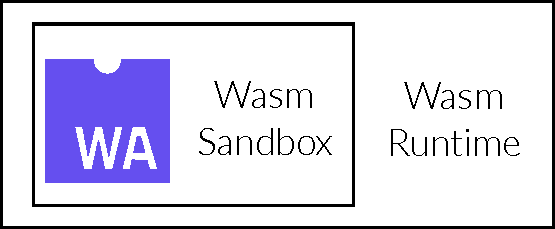
\includegraphics[width=\textwidth]{figures/security.pdf}
                \end{figure}
                \raggedleft
            \end{minipage}
            \heading{Full Portability}
            \begin{minipage}[t]{.30\textwidth}
            \vspace{-1em}
                \begin{figure}[t]
                \centering
                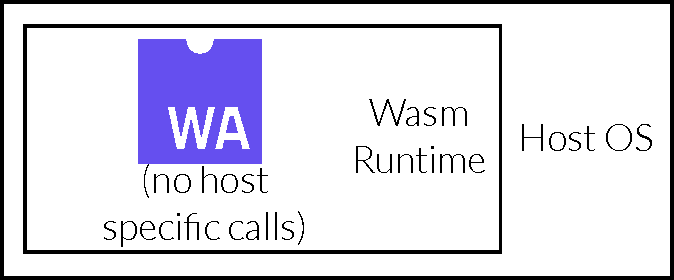
\includegraphics[width=\textwidth]{figures/portable.pdf}
                \end{figure}
                \raggedright
            \end{minipage}\hspace{0.05\textwidth}
            \begin{minipage}[t]{.65\textwidth}
                A Wasm module is just a binary format with no host-specific OS calls and it runs with limited, local, nondeterminism which sometimes might lead to unexpected behavior. Runtimes invent their own APIs.
            \end{minipage}
            \heading{Small Artifacts}
            \begin{minipage}[t]{.65\textwidth}
                \raggedright
                A Wasm module is also size-efficient when contrasted with containers since each module only has the runtime code and shares the runtime with other Wasm modules. The execution environments are still sandboxed from each other and can depend on different backends.
            \end{minipage}\hfill
            \begin{minipage}[t]{.30\textwidth}
            \vspace{-1em}
                \begin{figure}[t]
                \centering
                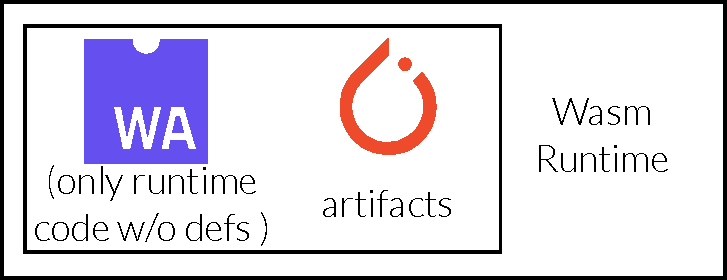
\includegraphics[width=\textwidth]{figures/size.pdf}
                \end{figure}
                \raggedleft
            \end{minipage}
        \end{block}
    
    
      \begin{block}{Python support for WebAssembly}
      
    
          \item \textbf { Compiling CPython to WASM : } The process of compiling Python to WebAssembly (Wasm) using Emscripten involves several key steps. 
    
          
          Emscripten is a powerful toolchain designed to compile C and C++ code into WebAssembly, and while it doesn't directly support Python, it can compile the CPython interpreter, enabling Python code to run in web browsers and other Wasm environments. 
    
          
          To begin, you need to install the Emscripten SDK, which provides essential tools like emcc, a C/C++ compiler that outputs Wasm. Next, you prepare your Python code, ensuring it is compatible with the WebAssembly environment by avoiding unsupported features. 
    
          
          Then, you use emcc to compile the CPython source code along with your Python files into a Wasm module. Optimization flags can be applied during this step to enhance performance or reduce file size. After compiling, you write JavaScript to load and interact with the Wasm module containing the Python interpreter. 
    
          
          Finally, you test and deploy the resulting WebAssembly application. 
    
            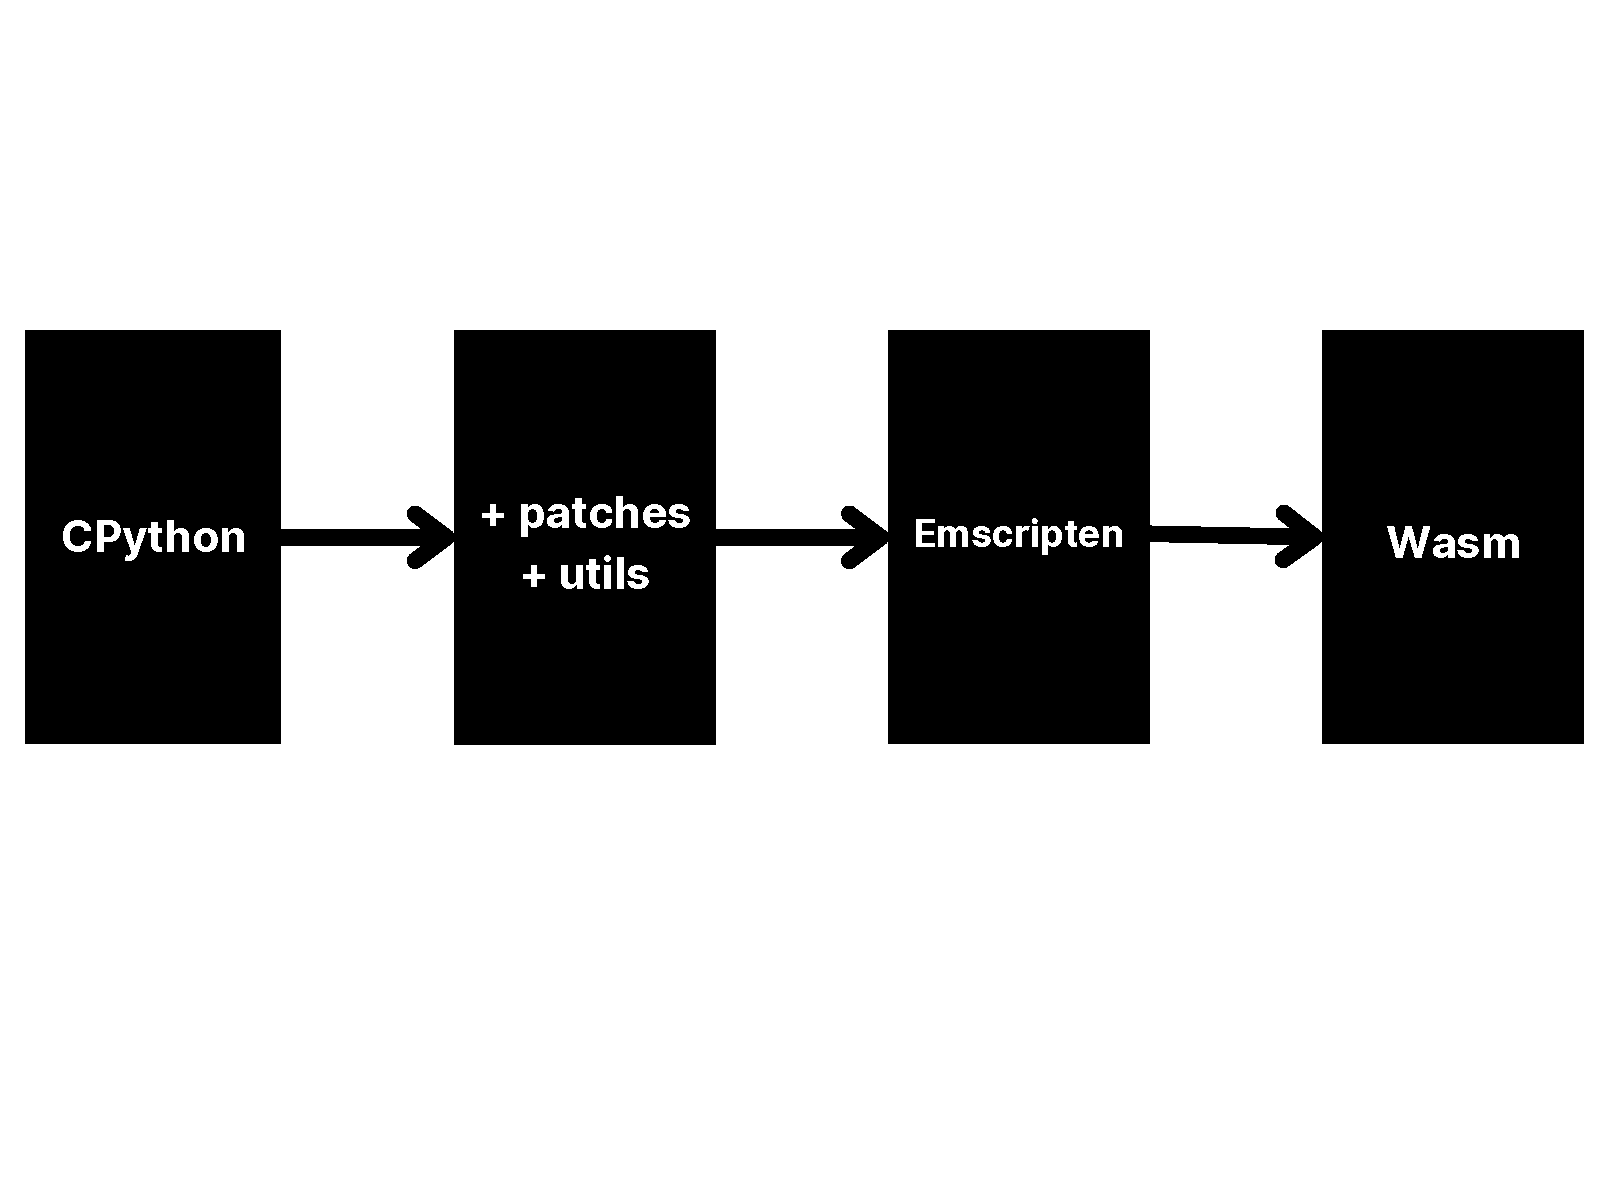
\includegraphics[width=1\linewidth]{figures/CPython.pdf}
    
    \end{block}
        \end{column}
            \separatorcolumn
        \begin{column}{\colwidth}
        
        \begin{block}{Python in the browser}
        \heading { PyScript - What is PyScript? and Architecture}
                \begin{minipage}[t]{\textwidth}
                    PyScript is a platform for running Python in modern web browsers. It's architecture has three core concepts:
                    \begin{itemize}
                    \item  A small, efficient and powerful kernel called PolyScript is the foundation upon which PyScript and plugins are built.
                    \item  A library called coincident that simplifies and coordinates interactions with web workers.
                    \item  The PyScript stack inside the browser is simple and clearly defined.

                    \end{itemize}
                    \newline
                    \centering
                    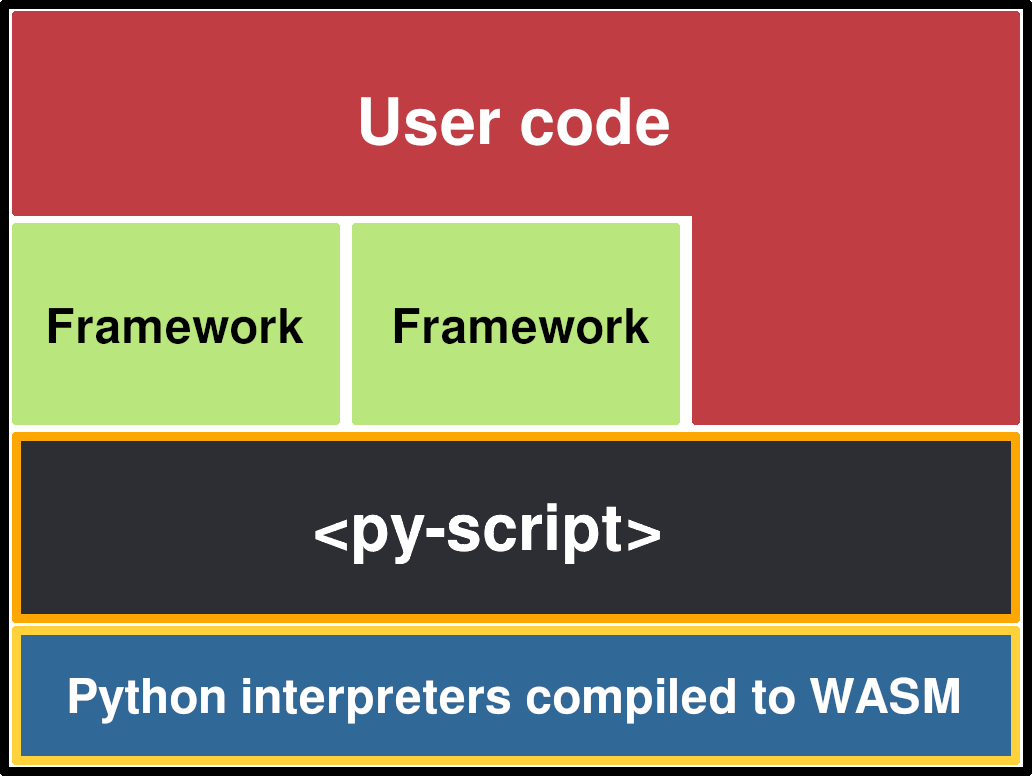
\includegraphics[\linewidth]{pyscript.png}
                    \begin{minted}[fontsize=\small]{html}
<html>
    <head>
        <link rel="stylesheet" href="https://pyscript.net/releases/2024.1.1/core.css">
        <script type="module" src="https://pyscript.net/releases/2024.1.1/core.js"></script>
        <title>PyScript Hello World</title>
    </head>
    <body>
        <section class="pyscript">
            This is the current date and time, as computed by Python:
            <script type="py">
                from pyscript import display
                from datetime import datetime
                now = datetime.now()
                display(now.strftime("%m/%d/%Y, %H:%M:%S"))
            </script>
        </section>
    </body>
</html>
\end{minted}
                    \end{minipage}
    
    
        \heading{Pyodide - What is Pyodide? and Architecture} 
    
                Pyodide is a Python distribution for the browser and Node.js based on WebAssembly/Emscripten.
    
                It makes it possible to install and run Python packages in the browser with micropip. Any pure Python package with a wheel available on PyPI is supported. Many packages with C extensions have also been ported for use with Pyodide. These include many general-purpose packages such as regex, PyYAML, lxml and scientific Python packages including NumPy, pandas, SciPy, Matplotlib, and scikit-learn.
                
                Pyodide comes with a robust Javascript ▤ Python foreign function interface so that you can freely mix these two languages in your code with minimal friction. This includes full support for error handling (throw an error in one language, catch it in the other), async/await, and much more.
                
                When used inside a browser, Python has full access to the Web APIs.
                
         \centering
                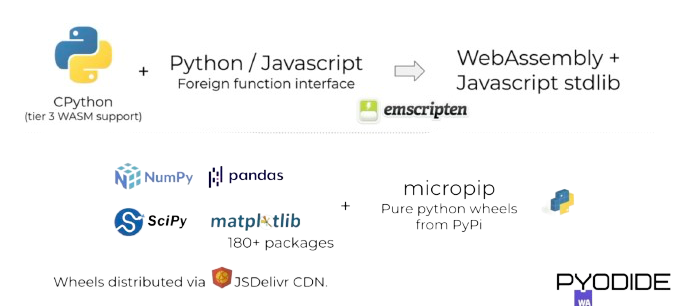
\includegraphics[width=0.7\linewidth]{figures/image.png}
        \end{block}
        \end{column}
        \separatorcolumn
            \begin{column}{\colwidth}
              \begin{block}{ Python in the serverless and cloud}

                 \heading{WebAssembly in Serverless with Spin} 
     \begin{minipage}[t]{\textwidth}
                   Spin is an open Source Developer Tool for building WebAssembly based serverless applications in just a few commands. \newline
                   

                   The Spin Python SDK is an experimental toolkit designed to help developers build serverless applications using Python, leveraging WebAssembly (Wasm) for deployment. This SDK is part of Fermyon's Spin framework, 

                    \begin{itemize}
                    \item The older version was created using Py2Wasm: A Python to WebAssembly compiler.

                    \item  The newer version is implemented with Compontentize.py: a tool to convert a Python application to a WebAssembly component

                    \end{itemize}
                 \end{minipage}
                    \begin{minted}[fontsize=\small]{python}
# Import necessary modules from the Spin SDK
from spin_sdk import http
from spin_sdk.http import Request, Response
from spin_sdk import llm


# Define a handler class for incoming HTTP requests
class IncomingHandler(http.IncomingHandler):
    # Define the method to handle incoming requests
    def handle_request(self, request: Request) -> Response:
        # Use the LLM to generate code for array implementation in multiple languages
        res = llm.infer_with_options(
            "llama2-chat",  # Specify the LLM model to use
            "write code to implement an Array in Java, C++, JavaScript and Rust",  # prompt
            llm.InferencingParams(temperature=0.5, max_tokens=1024)  # inference parameters
        )
        
        # Return the generated code as an HTTP response
        return Response(
            200,  # HTTP status code
            {"content-type": "text/plain"},  # Response headers
            bytes(res.text, "utf-8")  # Response body
        )
\end{minted}


                 \heading{Pyodide Support in Cloudflare Workers} 
     \begin{minipage}[t]{\textwidth}
                 Cloudflare Workers leverage Pyodide by integrating it directly into the Workers runtime, allowing developers to write serverless functions in Python. This integration utilizes Pyodide's WebAssembly-compiled Python interpreter and its foreign function interface to provide access to JavaScript APIs and dynamic linking of Python packages.

                    \begin{minted}[fontsize=\small]{python}
from js import Response
async def on_fetch(request, env):
    await env.FOO.put("bar", "baz")
    bar = await env.FOO.get("bar")
    return Response.new(bar) # returns "baz"
\end{minted}

                This example shows how bindings work in Python Workers: Put a key into Workers KV, and then read it.  \newline
                 \end{minipage}

   
                 \newline
                 \heading{Python support in WASI} 
     \begin{minipage}[t]{\textwidth}
                WASI is a system interface standard for WebAssembly. Through a combination of C compilers that can target WebAssembly and wasi-libc providing POSIX-compatible shims for WASI, it’s possible for CPython to run on a WASI host/runtime as a guest. \newline

                To build for WASI, you will need to cross-compile CPython. This requires a C compiler just like building for Unix as well as:
                
  \begin{itemize}
  
  \item C compiler that can target WebAssembly (for example, WASI SDK)

  \item WASI host/runtime (for example, Wasmtime)
  \end{itemize}
                 \end{minipage}

                    
                \end{block}

        
            \end{column}
                \separatorcolumn
\end{columns}
\end{frame}
\end{document}